\section{Kubernetes Cluster Autoscaler}
\label{section-gr:autoscaler}
\RestyleAlgo{ruled}

Σε αυτή την ενότητα, θα εκθέσουμε τον σχεδιασμό του Cluster Autoscaler, θα
περιγράψουμε τις κύριες αρχές λειτουργίας του, θα εντοπίσουμε τους περιορισμούς
του και θα προτείνουμε επεκτάσεις που θα επιτρέψουν την απρόσκοπτη λειτουργία
του με τοπικούς μόνιμους τόμους.


\subsection{Βασικοί Όροι}

Πριν περιγράψουμε τους αλγορίθμους λειτουργίας του Cluster Autoscaler, είναι
αρκετά σημαντικό να κατανοήσουμε ορισμένους θεμελιώδεις μηχανισμούς και την
ορολογία που χρησιμοποιεί.

\subsubsection{Ομάδα Κόμβων}

Ο Cluster Autoscaler χρησιμοποιεί την αφηρημένη έννοια ``\textit{ομάδα
      κόμβων}''. Μια ομάδα κόμβων δεν είναι ένα πραγματικό αντικείμενο του
      Kubernetes, αλλά μια αφηρημένη έννοια για ένα υποσύνολο κόμβων σε μια
      συστοιχία. Οι κόμβοι που ανήκουν στην ίδια ομάδα κόμβων αναμένεται να
      έχουν τους ίδιους πόρους (CPU, μνήμη) και να μοιράζονται αρκετές κοινές
      ιδιότητες, όπως ετικέτες και taints. Ωστόσο, μπορούν ακόμη να
      διαφοροποιούνται σε ορισμένες λεπτομέρειες, π.χ. μπορεί να ανήκουν σε
      διαφορετικές ζώνες διαθεσιμότητας.

Κάθε ομάδα κόμβων έχει τις ακόλουθες σημαντικές ιδιότητες:
\begin{itemize}
      \tightlist
      \item \co{minSize}: το ελάχιστο μέγεθος της ομάδας κόμβων.
      \item \co{maxSize}: το μέγιστο μέγεθος της ομάδας κόμβων.
      \item \co{targetSize}: το επιθυμητό μέγεθος της ομάδας κόμβων.
\end{itemize}

\subsubsection{Η Διεπαφή \texttt{CloudProvier}}

Ο Cluster Autoscaler λειτουργεί με διάφορους παρόχους cloud, π.χ. με το GCE,
AWS, κ.λπ. Για να το επιτύχει αυτό, ορίζει δύο σημαντικές διεπαφές που κάθε
πάροχος νέφους που επιθυμεί την ενσωμάτωση των υπηρεσιών του με τον Cluster
Autoscaler πρέπει να υλοποιήσει:
\begin{itemize}
      \tightlist
      \item Η διεπαφή \co{CloudProvider}: περιέχει πληροφορίες διαμόρφωσης και
            λειτουργίες για την αλληλεπίδραση με τον πάροχο του νέφους.
      \item Η διεπαφή \co{NodeGroup}: περιέχει πληροφορίες διαμόρφωσης και
            λειτουργίες για τον έλεγχο μίας ομάδας κόμβων.
\end{itemize}

Η διεπαφή \co{NodeGroup} βασίζεται στην έννοια \textit{ομάδα κόμβων}, την οποία
εξηγήσαμε προηγουμένως. Κάθε πάροχος νέφους μπορεί να επιλέξει τη δική του
ερμηνεία για το τι είναι ομάδα κόμβων στην υπηρεσία του, αρκεί να συμμορφώνεται
με τον ορισμό της έννοιας.

Για παράδειγμα, στην περίπτωση του AWS EKS, η υλοποίηση του \co{NodeGroup}
αντιστοιχίζει την κάθε ομάδα κόμβων σε μια ομάδα αυτόματης κλιμάκωσης (ASG) του
AWS. Ο Cluster Autoscaler δεν γνωρίζει την υποκείμενη υλοποίηση κάθε παρόχου
νέφους.

\subsubsection{Η Διεπαφή \texttt{ClusterSnapshot}}

Ο Cluster Autoscaler εκτελεί προσομοιώσεις στη συστοιχία για τη λήψη αποφάσεων.
Για να το επιτύχει αυτό, λαμβάνει ένα στιγμιότυπο της τρέχουσας συστοιχίας
χρησιμοποιώντας τη διεπαφή \texttt{ClusterSnapshot}, προσθέτει ή αφαιρεί κόμβους
στο στιγμιότυπο και προσομοιώνει τις αποφάσεις χρονοδρομολόγησης στο
τροποποιημένο στιγμιότυπο.  Ένα στιγμιότυπο συστοιχίας περιέχει μια παγωμένη
εικόνα των κόμβων της συστοιχίας ως καθώς και των Pods που εκτελούνται σε κάθε
κόμβο της. Σημειώνουμε ότι τα PVCs και τα PVs της συστοιχίας δεν περιέχονται στη
συστοιχία, αντ' αυτού το VolumeBinding plugin τα ζητά από τον  API Server και
ελέγχει αν ένα Pod μπορεί να τοποθετηθεί σε έναν κόμβο βάσει τον τόμων του.

\subsubsection{Η Διεπαφή \texttt{PredicateChecker}}

Ο Cluster Autoscaler ορίζει τη διεπαφή \co{PredicateChecker}, η οποία
προδιαγράφει μεθόδους που ελέγχουν αν όλα τα απαιτούμενα predicates / κριτήρια
επιτυγχάνουν για δεδομένο Pod και κόμβο. Ένα predicate είναι ισοδύναμο με ένα
πρόσθετο \co{Filter} και χρησιμοποιείται για το φιλτράρισμα των κόμβων που δεν
μπορούν να εκτελέσουν ένα Pod. Ουσιαστικά, με τον PredicateChecker ο Cluster
Autoscaler ελέγχει αν ένα Pod μπορεί να τρέξει σε έναν κόμβο. Η υλοποίηση
\texttt{SchedulerBasedPredicateChecker} της διεπαφής, κάνει χρήση του κώδικα του
Scheduler για να ελέγξει κατά τις προσομοιώσεις του Cluster Autoscaler αν ένα
Pod μπορεί να τρέξει σε έναν κόμβο.

\subsubsection{Οι Διεπαφές \texttt{Esitmator} \&  \texttt{Strategy}} Ο Autoscaler ορίζει
δύο διεπαφές που χρησιμοποιούνται στη διαδικασία κλιμάκωσης:
\begin{itemize}
      \tightlist
      \item \co{Estimator}: διεπαφή για τον υπολογισμό του αριθμού των κόμβων
            ενός δεδομένου τύπου που απαιτούνται για τον προγραμματισμό
      \item \co{Strategy}: διεπαφή για τη λήψη απόφασης σχετικά με την καλύτερη
            επιλογή κλιμάκωσης.
\end{itemize}

Ο Estimator που χρησιμοποιείται επί του παρόντος από τον Autoscaler είναι ο
\en{\co{BinPackingNodeEstimator}} και υλοποιεί τον First Fit Decreasing bin
packing αλγόριθμο.


\subsubsection{Πρότυπος Κόμβος}
\label{section-gr:design-template}

Ο Cluster Autoscaler  για να εκτελέσει το προσομοιώσεις του, κατασκευάζει έναν
πρότυπο κόμβο για κάθε ομάδα κόμβων. Ένας πρότυπος κόμβος, όπως υποδηλώνει το
όνομα, είναι μια αναπαράσταση του πώς θα έμοιαζε ένας νέος κόμβος της ομάδας
κόμβων μόλις μετά την προσθήκη του στη συστοιχία.

O Cluster Autoscaler προσπαθεί να δημιουργήσει έναν πρότυπο κόμβο μιας ομάδας
κόμβων ως εξής:
\begin{enumerate}
      \tightlist
      \item Αρχικά, αναζητά έναν Ready και χρονοδρομολογήσιμο κόμβο της ομάδας
            κόμβων στη συστοιχία.
      \item Εάν το προηγούμενο βήμα απέτυχε, αναζητά ένα πρότυπο στη μνήμη
            cache του.
      \item Εάν το προηγούμενο βήμα απέτυχε, καλεί το μεταγλωττισμένο πρόσθετο
            του παρόχου νέφους για τη δημιουργία ενός προτύπου για τη
            συγκεκριμένη ομάδα κόμβων.
      \item Εάν το προηγούμενο βήμα απέτυχε, αναζητά  τυχόν Unready ή μη
            χρονοδρομολογήσιμους κόμβους της  ομάδας κόμβων στη συστοιχία και
            τον χρησιμοποιεί για τη δημιουργία του προτύπου.
\end{enumerate}

Οι κόμβοι του κατασκευασμένου προτύπου \textit{απολυμαίνονται}: η
\textit{απολύμανση} ενός κόμβου είναι ένας μηχανισμός που αφαιρεί άσχετες ή
ανεπιθύμητες λεπτομέρειες από το κατασκευασμένο πρότυπο κόμβου, όπως, το όνομα
του κόμβου, συγκεκριμένες ετικέτες, κ.λπ.



\subsubsection{Χρησιμοποίηση Κόμβου}

% transl: χρησιμοποίηση transl: eviction transl: πρότυπος κόμβος transl: cloud
% provider transl: ομάδα κόμβων transl: Απολύμανση transl: χρησιμοποίηση transl:
% scale-up down transl: χρονοδρομολογήσιμος κόμβος και μη , το ίδιο για Pods

Όσον αφορά την κλιμάκωση προς τα κάτω, ο Autoscaler ενεργεί με βάση τη
\textit{χρησιμοποίηση} ενός κόμβου, η οποία υπολογίζεται χρησιμοποιώντας τα
αιτήματα πόρων των Pods που εκτελούνται στον κόμβο και όχι σε πραγματικές
(ζωντανές) μετρήσεις χρήσης πόρων.

Κάθε κόμβος της συστοιχίας μπορεί να διαθέτει πολλαπλούς πόρους, όπως CPU, μνήμη
κ.λπ. Ο Cluster Autoscaler υπολογίζει τη χρησιμοποίηση κάθε κόμβου στη
συστοιχία. Για ένα συγκεκριμένο πόρο, η χρησιμοποίηση των κόμβων είναι το
άθροισμα των αιτήσεων των Pods που εκτελούνται στον κόμβο για τον πόρο δια την
διαθέσιμη ποσότητα του  πόρου στον κόμβο.  Η χρησιμοποίηση είναι ένας αριθμός
float, με εύρος από 0 έως 1, όπου το 1 υποδηλώνει πλήρη χρησιμοποίηση και το 0
καθόλου χρησιμοποίηση.

\subsection{Ο Κύριος Βρόχος}
Ο Cluster Autoscaler τρέχει διαρκώς τον \textit{κύριο βρόχο},  που εκτελεί 2 βασικές
λειτουργίες στη συστοιχία:
\begin{itemize}
      \tightlist
      \item \textit{Κλιμάκωση προς τα πάνω}: προσθήκη νέων κόμβων στη συστοιχία
            για να βοηθηθούν τα Pods που δεν μπορούν να χρονοδρομολογηθούν.
      \item \textit{Κλιμάκωση προς τα κάτω}: αφαίρεση μη απαραίτητων κόμβων από
            τη συστοιχία.
\end{itemize}

\subsection{Κλιμάκωση Προς τα Κάτω}
Σε κάθε επανάληψη του κύριου βρόχου, εάν δεν επιχειρήθηκε κλιμάκωση προς τα
πάνω, ο Cluster Autoscaler εκτελεί τη διαδικασία αξιολόγησης της κλιμάκωσης προς
τα κάτω.

% transl: unneeded node
Η αξιολόγηση της κλιμάκωσης προς τα κάτω αποτελείται από δύο μέρη:
\begin{enumerate}
      \tightlist
      \item \textit{Ενημέρωση περιττών κόμβων}:  υπολογίζει ποιοι κόμβοι της
            συστοιχίας είναι περιττοί και για πόσο χρονικό διάστημα.
      \item \textit{Προσπάθεια κλιμάκωσης προς τα κάτω}: προσπαθεί να μειώσει
            την κλίμακα της συστοιχίας προς τα κάτω αφαιρώντας περιττούς
            κόμβους.
\end{enumerate}

\begin{figure}[H]
      \centering
      \makebox[\textwidth][c]{
            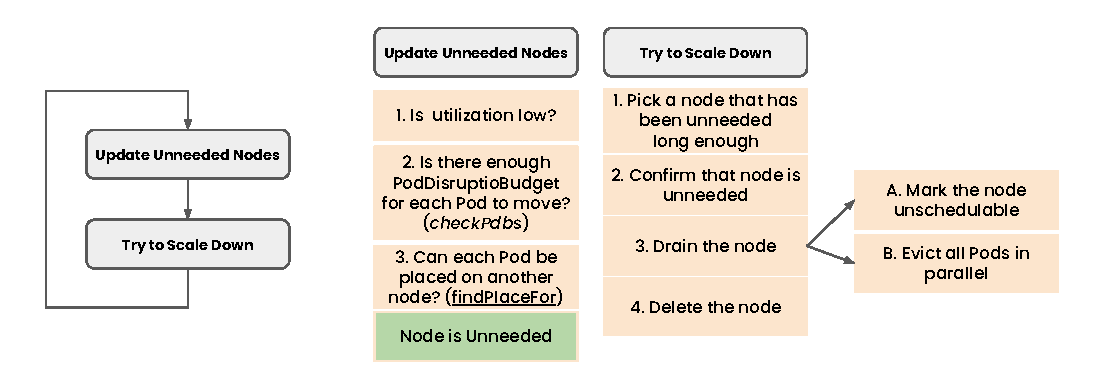
\includegraphics[width=1.1\textwidth]{resources/autoscaler-scale-down-process.pdf}
      }
      \caption{Cluster Autoscaler: Διαδικασία κλιμάκωσης προς τα κάτω}
      \label{figure:gr-autoscaler-scale-down}
\end{figure}

\subsubsection{Διαδικασία Ενημέρωσης Περιττών Κόμβων}

Η διαδικασία \textit{ενημέρωσης περιττών κόμβων} υπολογίζει ποιοι κόμβοι της
συστοιχίας είναι περιττοί και ενημερώνει την εσωτερική κατάσταση του Autoscaler με τη
χρονική διάρκεια για την οποία έχουν παραμείνει περιττοί.

Ένας κόμβος θεωρείται \textit{περιττός} εάν πληρούνται όλα τα ακόλουθα κριτήρια:
\begin{itemize}
      \tightlist
      \item H μετρική της χρησιμοποίησης των πόρων του κόμβου είναι κάτω από ένα
            συγκεκριμένο κατώφλι. Σε αυτή την περίπτωση ο κόμβος αναφέρεται ως
            \textit{``υποχρησιμοποιούμενος''}.
      \item Τα Pods που εκτελούνται στον κόμβο μπορούν να εκδιωχθούν, δηλαδή η
            εκδίωξή τους δεν περιορίζεται από κάποιο PodDisruptionBudget.
      \item Τα Pods που εκτελούνται στον κόμβο μπορούν να μετακινηθούν σε
            διαφορετικό κόμβο της συστοιχίας.
\end{itemize}

% lang: unremovable, περιττος, υποχρησιμοποιούμενος
Εάν ένας κόμβος δεν ικανοποιεί τα παραπάνω κριτήρια, αποκαλείται
\textit{αναφαίρετος}, αφού δεν μπορεί να αφαιρεθεί από τη συστοιχία.

Για να καθορίσει αν ένας υποχρησιμοποιούμενος κόμβος είναι περιττός, ο Autoscaler
εκτελεί τα εξής βήματα:
\begin{enumerate}
      \tightlist
      \item Υπολογίζει τα Pods που πρέπει να μετακινηθούν σε περίπτωση που ο
            κόμβος αφαιρεθεί.
      \item Ελέγχει εάν υπάρχουν PodDisruptionBudgets που εμποδίζουν την έξωση
            οποιουδήποτε Pod. Εάν ναι, ο κόμβος δεν μπορεί να αφαιρεθεί.
      \item Καλεί τη μέθοδο \co{FindPlaceFor()} για να βρει θέση για τα Pods σε
            ένα διαφορετικό κόμβο. Η \co{FindPlaceFor()} χρησιμοποιεί την
            διεπαφή \en{\co{SchedulerBasedPredicateChecker}} για να καθορίσει αν
            το Pod μπορεί να είναι τοποθετηθεί σε οποιονδήποτε άλλο κόμβο.
            Ελέγχει αν το Pod μπορεί να χωρέσει σε έναν κόμβο λόγω οποιωνδήποτε
            άλλων περιορισμών χρονοδρομολόγησης (CPU, μνήμη), καθώς και αν ο οι
            τόμοι του Pod μπορούν να προσπελαστούν από τον κόμβο.
\end{enumerate}

\subsubsection{Διαδικασία Προσπάθειας Κλιμάκωσης Προς Τα Κάτω}


% TODO: να παραπεμψω προς το πίνακα, μήπως  πρέπει να πάει καπου αλλου;
Εάν ένας \textit{Ready} κόμβος παραμείνει περιττός για διάστημα μεγαλύτερο από
το \en{\co{scaleDownUnneededTime}} ή ένας \textit{Unready} κόμβος παραμείνει
περιττός για διάστημα μεγαλύτερο από το \en{\co{scaleDownUnreadyTime}} (δείτε
τον Πίνακα \ref{table:symbolic-names-autoscaler} στο αγγλικό μέρος της εργασίας
για τους ορισμούς αυτών των συμβολικών ονομάτων), ο Cluster Autoscaler θα
θεωρήσει τον κόμβο ως υποψήφιο για διαγραφή.

Ο Cluster Autoscaler κάνει διάκριση μεταξύ μη κενών και κενών κόμβων:
\begin{itemize}
      \tightlist
      \item \textit{Κενοί κόμβοι}: κόμβοι που εκτελούν \textit{μονάχα} DaemonSet
            Pods. O Autoscaler αφαιρεί τους κενούς κόμβους μαζικά.
      \item \textit{Non-empty nodes}: κόμβοι που δεν εκτελούν μόνο DaemonSet
            Pods. O Autoscaler αφαιρεί τους μη κενούς κόμβους έναν προς έναν προκειμένου
            να μη δημιουργηθούν μη χρονοδρομολογήσιμα Pods.
\end{itemize}


\paragraph*{Διαγραφή κόμβου}

Η διαγραφή κόμβου εκτελείται ως εξής:
\begin{enumerate}
      \tightlist
      \item Βάζει ένα taint  \co{ToBeDeletedByClusterAutoscaler:NoSchedule} στον
            κόμβο, ουσιαστικά χαρακτηρίζοντας τον κόμβο ως unschedulable.
      \item Ξεκινά τη διαδικασία drain του κόμβου, εκδιώκοντας παράλληλα όλα τα
            Pods του κόμβου. Εάν κάποιο Pod δεν μπορεί να εκδιωχθεί λόγω κάποιου
            PDB, επαναλαμβάνει την προσπάθεια έως ότου παρέλθει το χρονικό
            διάστημα \en{\co{MaxPodEvictionTimeout}}.
      \item Όταν όλα τα Pods εκδιωχθούν επιτυχώς, ζητά από τον πάροχο νέφους
            να διαγράψει τον κόμβο.
\end{enumerate}

\subsection{Κλιμάκωση Προς τα Πάνω}

Εάν η συστοιχία έχει Pods που δεν μπορούν να χρονοδρομολογηθούν, ο \en{Cluster
      Autoscaler} θα προσπαθήσει να τα βοηθήσει κλιμακώνοντας προς τα πάνω τη
      συστοιχία, δηλαδή προσθέτοντας νέους κόμβους. Η κλιμάκωση προς τα πάνω
      μίας συστοιχίας, επιτυγχάνεται αυξάνοντας το επιθυμητό μέγεθος
      (\co{targetSize}) κάποιων ομάδων κόμβων. Εάν έχουν διαμορφωθεί πολλαπλές
      ομάδες κόμβων στη συστοιχία, τότε πρέπει να αποφασίσει τα εξής:
\begin{itemize}
      \tightlist
      \item Ποια ομάδα κόμβων μπορεί να τρέξει το μη χρονοδρομολογήσιμο Pod.
      \item Πόσοι κόμβοι της κάθε ομάδας κόμβων απαιτούνται.
      \item Στην περίπτωση που η κλιμάκωση προς τα πάνω διαφορετικών ομάδων
            κόμβων είναι εφικτή, ποια ομάδα κόμβων θα κλιμακωθεί.
\end{itemize}

Όταν το επιθυμητό μέγεθος μιας ομάδας κόμβων αυξάνεται, ο πάροχος του νέφους θα
δημιουργήσει νέους κόμβους, ο οποίοι θα ενταχθούν στη συστοιχία Kubernetes και ο
χρονοδρομολογητής θα αναθέσει σταδιακά τα μέχρι πρότινος μη χρονοδρομολογήσιμα
Pods στους νέους κόμβους.

\paragraph*{Επιλογές κλιμάκωσης}
Για να αποφασίσει αν η αύξηση της κλίμακας μιας ομάδας κόμβων θα βοηθήσει τα μη
χρονοδρομολογήσιμα Pods, ο Cluster Autoscaler εκτελεί τα εξής βήματα:
\begin{enumerate}
      \tightlist
      \item Λαμβάνει ένα στιγμιότυπο της συστοιχίας
      \item Προσθέτει έναν πρότυπο κόμβο της ομάδας κόμβων στο στιγμιότυπο
      \item Προσομοιώνει, χρησιμοποιώντας τον
            \co{SchedulerBasedPredicateChecker}, αν το μη χρονοδρομολογήσιμο Pod
            μπορεί να χρονοδρομολογηθεί στο τροποποιημένο στιγμιότυπο της
            συστοιχίας.
      \item Εάν η προσομοίωση δείξει ότι το Pod μπορεί να χρονοδρομολογηθεί, ο
            Cluster Autoscaler θα χρησιμοποιήσει τον
            \co{BinPackingNodeEstimator} για να υπολογίσει πόσοι κόμβοι της
            συγκεκριμένης ομάδας κόμβων απαιτούνται.
\end{enumerate}

Η δυνατότητα για κλιμάκωση μιας συγκεκριμένης ομάδας κόμβων μαζί με τον αριθμό
των κόμβων της ομάδας που απαιτούνται, αναφέρεται ως ``\textit{επιλογή
κλιμάκωσης}''.

\paragraph*{Στρατηγική κλιμάκωσης}
Εάν υπάρχουν πολλαπλές επιλογές κλιμάκωσης, ο Cluster Autoscaler θα αποφασίζει
ποια είναι η καλύτερη χρησιμοποιώντας τη διεπαφή \co{Strategy}. Υπάρχουν
διάφορες στρατηγικές και ο τελικός χρήστης μπορεί να ρυθμίσει τον Autoscaler ώστε να να
χρησιμοποιεί την επιθυμητή, π.χ. την επιλογή με το μικρότερο κόστος, την τυχαία
στρατηγική κ.λπ.


\subsection{Ελλείψεις \& Προτεινόμενες Επεκτάσεις}

\subsubsection{Κλιμάκωσης Προς τα Κάτω: Οι Μόνιμοι Τόμοι του Rok Μετακινούνται}
\label{section-gr:design-autoscaler-unpinned}

Κατά την αξιολόγηση της αφαίρεσης ενός κόμβου, ο Autoscaler προσπαθεί να βρει θέση για
τα Pods που εκτελούνται στον κόμβο σε άλλους κόμβους της συστοιχίας. Για τον
σκοπό αυτό, καλεί τη μέθοδο \texttt{FindPlaceFor()}, η οποία με τη σειρά της
αξιοποιεί τις μεθόδους της διεπαφής \texttt{PredicateChecker} για να διαπιστώσει
αν ένα Pod ταιριάζει σε έναν κόμβο. Η υλοποίηση της διεπαφής
\texttt{SchedulerBasedPredicateChecker}, εκτελεί τη μέθοδο \texttt{Filter()} του
πρόσθετου VolumeBinding για να ελέγξει αν οι τόμοι του Pod μπορούν να
προσπελαστούν από άλλον κόμβο.

Τα PV της κλάσης αποθήκευσης του Rok  έχουν node affinity  που ταιριάζει μόνο με
τον κόμβο στον οποίο ο τόμος βρίσκεται. Δεδομένου ότι το node affinity των τόμων
δεν ταιριάζει με κανέναν άλλο κόμβο στη συστοιχία, ο Autoscaler θα θεωρήσει ότι το Pod
και ο τόμος του δεν μπορούν να μετακινηθούν σε διαφορετικό κόμβο,
χαρακτηρίζοντας έτσι το τρέχοντα κόμβο ως αναφαίρετο. Ο Autoscaler, και ο
\en{\co{SchedulerBasedPredicateChecker}} ειδικότερα, δεν γνωρίζουν ότι οι τόμοι της
κλάσης Rok διαθέτουν έναν μηχανισμό που θα λάβει ένα στιγμιότυπο και θα μπορεί
να τους ανακτήσει σε διαφορετικό κόμβο (διαδικασία unpinning \& pinning, βλ.
ενότητα ~\ref{section:gr-rok-volume-pinning}).

Προτείνουμε την επέκταση του Autoscaler ώστε να προσομοιώνει τους τόμους Rok ως unpinned
(σαν να μην έχουν node affinity) κατά την αξιολόγηση μιας κλιμάκωσης προς τα
κάτω (τότε, και μόνο τότε - σε άλλες περιπτώσεις οι τόμοι διατηρούν το node
affinity τους). Με αυτή την επέκταση, ο Autoscaler θα αντιλαμβάνεται ότι οι τόμοι Rok
μπορούν να μετακινηθούν οπουδήποτε στη συστοιχία και ο κόμβος μπορεί να
αφαιρεθεί με ασφάλεια.

\subsubsection{Κλιμάκωση Προς Τα Κάτω: Συνεργασία με τον Μηχανισμό Rok CSI Guard}

Στο πλαίσιο του μηχανισμού προστασίας των τόμων του Rok (βλ. ενότητα
\ref{section:background-gr-rok-csi-guard}), δημιουργούμε ένα αντικείμενο
\texttt{Deployment} για κάθε κόμβο της συστοιχίας, το οποίο δημιουργεί ένα Pod
ανά κόμβο (Rok CSI Guard) με αυστηρό node affinity που ταιριάζει μόνο με τον
κόμβο που προστατεύει. Ο Autoscaler θα προσπαθήσει να βρει κάποιον κόμβο για να
μετακινήσει το Pod. Ωστόσο, επειδή το Pod έχει  node affinity ταιριάζει μόνο
στον τρέχοντα κόμβο δεν μπορεί να μετακινηθεί αλλού, και ως εκ τούτου ο Autoscaler θα
χαρακτηρίσει τον τρέχοντα κόμβο ως αναφαίρετο. Φυσικά, το Pod θα αφαιρεθεί
εντελώς από τον Rok Operator μόλις ο κόμβος αφαιρεθεί, αλλά ο Autoscaler δεν το γνωρίζει
αυτό.

Επιπλέον, ο Autoscaler θα ελέγξει το PDB του Guard Pod. Το PDB του Rok CSI Guard Pod
έχει ρυθμιστεί ώστε να προκαλεί την αποτυχία τυχόν εκδιώξεων. Ο Autoscaler θα το
παρατηρήσει αυτό, θα θεωρήσει ότι το Guard Pod δεν θα μπορέσει να εκδιωχθεί με
ασφάλεια, και θα χαρακτηρίσει τον κόμβο αναφαίρετο. Ο Autoscaler δεν γνωρίζει ότι το PDB
διαχειρίζεται από τον Rok Operator και ότι θα αφαιρεθεί μόλις ξεκινήσει η
κλιμάκωση προς τα κάτω του κόμβου και οι  τοπικοί τόμοι του Rok  στον κόμβο
γίνουν unpinned.

Προτείνουμε την επέκταση του Autoscaler έτσι ώστε να μην προσπαθεί να βρει θέση για την
Guard Pod. Επιπλέον, επεκτείνουμε την Autoscaler ώστε να αγνοεί το PDB του Guard Pod
όταν κατά την αξιολόγηση της δυνατότητας αφαίρεσης ενός κόμβου. Παρόλα αυτά, ο
Autoscaler θα γνωρίζει ότι ο Pod υπάρχει και θα αρχίσει να εκδιώκει (evict) το Guard Pod
όταν κάνει drain τον κόμβο.

Για να γίνουν τα πράγματα πιο κατανοητά, ακολουθεί η διαδικασία που θα
πραγματοποιείται με το νέο σχεδιασμό:

\begin{enumerate}
      \tightlist
      \item Ο Autoscaler αξιολογεί έναν κόμβο για αφαίρεση:
            \begin{enumerate}
                  \item Ελέγχει αν το PDB επιτρέπει την εκδίωξη των Pods που
                        εκτελούνται στον κόμβο, αλλά αγνοεί το PDB του Guard
                        Pod.
                  \item Προσπαθεί να βρει θέση για κάθε Pod σε διαφορετικό
                        κόμβο, αλλά αγνοεί το Guard Pod.
            \end{enumerate}
      \item Ο Autoscaler αποφασίζει να αφαιρέσει τον κόμβο.
      \item Ο Autoscaler προσθέτει το taint διαγραφής στον κόμβο, χαρακτηρίζοντάς τον
            ουσιαστικά ως ως μη χρονοδρομολογήσιμο.
      \item Ο Autoscaler αποστέλλει αιτήματα εκδίωξης για κάθε Pod στον API Server.
      \item Η εκδίωξη όλων των Pods --εκτός από το Guard Pod-- είναι επιτυχής.
      \item Ο Autoscaler συνεχίζει να προσπαθεί εκ νέου να εκδιώξει το Guard Pod, αλλά ο
            API Server απαντά ότι η εκδίωξη δεν επιτρέπεται λόγω του ρυθμισμένου
            PDB.
      \item Ο ελεγκτής CSI του Rok παρατηρεί ότι ο κόμβος είναι μη
            χρονοδρομολογήσιμος και ότι κανένα Pod δεν προσαρτά
            τους τόμους, οπότε αρχίζει να τους τους κάνει unpin.
      \item Ο ελεγκτής CSI του Rok ολοκληρώνει το unpin των τόμων και αφαιρεί το
            node affinity των αντίστοιχων PV.
      \item Ο Rok Operator αφαιρεί το PodDisruptionBudget του Guard Pod.
      \item Το αίτημα του Autoscaler για την έξωση του Guard Pod τελικά πετυχαίνει (αφού
            το PDB αφαιρέθηκε).
      \item Ο Autoscaler ζητά από τον πάροχο νέφους να διαγράψει τον κόμβο.
      \item Ο Rok Operator αφαιρεί το Rok CSI Guard Deployment του κόμβου που
            μόλις αφαιρέθηκε.
\end{enumerate}

\subsubsection{Κλιμάκωση Προς τα Κάτω: Διαθέσιμος Αποθηκευτικός Χώρος}

Ο Autoscaler θα πρέπει ελέγχει εάν οι τόμοι της κλάσης αποθήκευσης Rok ενός Pod μπορούν
να χωρέσουν σε έναν κόμβο ως προς τον απαιτούμενο αποθηκευτικό χώρο  κατά την
αξιολόγηση της κλιμάκωσης προς τα κάτω. Όπως έχουμε εξηγήσει, ο Autoscaler χρησιμοποιεί
τη διεπαφή \texttt{SchedulerBasedPredicateChecker} προκειμένου να ελέγξει αν ένα
Pod χωράει σε έναν κόμβο, η οποία --μεταξύ άλλων-- καλεί τη μέθοδο
\co{Filter()} του πρόσθετου VolumeBinding.

Προτείνουμε την επέκταση της μεθόδου \co{Filter} του VolumeBinding προσθέτου του
SchedulerBasedPredicateChecker , έτσι ώστε όταν καλείται να ελέγξει αν ένα Pod
μπορεί να μετακινηθεί σε διαφορετικό κόμβο να λαμβάνει υπόψη αν υπάρχει αρκετός
διαθέσιμος αποθηκευτικός χώρος στον κόμβο για να μεταφερθούν εκεί οι τόμοι του
Pod.

Επιπλέον, δεδομένου ότι η δημιουργία στιγμιότυπων και η μετακίνηση ενός τόμου
είναι μια διαδικασία που κοστίζει σε χρόνο, θα θέλαμε ο Autoscaler να μην αφαιρεί
κόμβους που έχουν υψηλή χρησιμοποίηση της αποθήκευσης, κατά παρόμοιο τρόπο με
το πως χειρίζεται τη χρησιμοποίηση της CPU και τη μνήμης. Για να το επιτύχουμε
αυτό, προτείνουμε την επέκταση του Autoscaler με μία νέα μετρική, που ονομάζεται
``\textit{χρησιμοποίηση αποθηκευτικού χώρου}'', και ορίζεται ως ο λόγος του
χρησιμοποιούμενου αποθηκευτικού χώρου προς τη μέγιστη αποθηκευτική ικανότητα του
κόμβου. Ο Autoscaler θα συγκρίνει αυτή τη μετρική με ένα κατώφλι, το οποίο μπορεί να
διαμορφωθεί από τον διαχειριστή της συστοιχίας μέσω μίας σημαίας στον Autoscaler. Εάν η
χρήση του αποθηκευτικού χώρου είναι πάνω από το κατώφλι, ο κόμβος θα θεωρείται
αναφαίρετος.

% transl: Αναφαίρετος

\subsubsection{Κλιμάκωση Προς τα Κάτω: Οι Unready Κόμβοι Να Μην Αφαιρούνται}

Ένας κόμβος με κατάσταση \co{Ready} μπορεί να γίνει \co{Unready} (ή
\co{NotReady}) εάν προκύψει κάποιο πρόβλημα. Οι συνήθεις λόγοι περιλαμβάνουν την
έλλειψη πόρων στον κόμβο, ένα πρόβλημα με το kubelet, ένα σφάλμα που σχετίζεται
με τον kube-proxy ή ένα πρόβλημα δικτύωσης.

Ο Autoscaler  αφαιρεί κάθε περιττό κόμβο σε κατάσταση Unready μόλις παρέλθει το
\en{\texttt{scaleDownUnreadyTime}} διάστημα. Αυτό είναι πρόβλημα, δεδομένου ότι
οι τοπικοί τόμοι που βρίσκονται στον κόμβο θα χαθούν μόνιμα. Ο Autoscaler δεν πρέπει να
αφαιρεί Unready κόμβους. Αντιθέτως, οι κόμβοι πρέπει να παραμένουν στη συστοιχία,
έτσι ώστε ένας διαχειριστής να εκτελέσει κατάλληλες ενέργειες για την ανάκαμψη
από της κατάσταση Unready.

Προτείνουμε την επέκταση του Autoscaler με μια σημαία για τη ρητή απενεργοποίηση
της μείωση της κλίμακας για τους κόμβους που βρίσκονται σε κατάσταση
\co{Unready}, και να θεωρεί αυτούς τους κόμβους ως αναφαίρετους όταν
απενεργοποιείται η κλιμάκωση προς τα κάτω  για τους Unready κόμβους.


\subsubsection{Κλιμάκωση Προς τα Πάνω: Χωρητικότητα Αποθήκευσης}

Ο Autoscaler δεν γνωρίζει πόσος τοπικός αποθηκευτικός χώρος θα είναι διαθέσιμος όταν
ένας νέος κόμβος προστεθεί στη συστοιχία. Ο πρότυπος κόμβος που δημιουργείται
από έναν ζωντανό κόμβο  περιέχει πληροφορίες μονάχα για τον εναπομείναντα
ελεύθερο αποθηκευτικό χώρο (ο οδηγός αποθήκευσης αναφέρει την τιμή αυτή ως
annotation στο Node αντικείμενο) . Χρειαζόμαστε έναν μηχανισμό για να γνωρίζουμε
πόσο ελεύθερο αποθηκευτικό χώρο θα έχει ένας νέος κόμβος μιας ομάδας κόμβων
μόλις προστεθεί, τον οποίο ο Autoscaler θα το λαμβάνει υπόψη στις προσομοιώσεις
του.

\paragraph*{Αναφορά μεγίστης χωρητικότητας}

Υποθέτοντας ότι όλοι οι κόμβοι σε μια ομάδα κόμβων έχουν την ίδια διαμόρφωση
δίσκου και την ίδια μέγιστη χωρητικότητα αποθήκευσης, μπορούμε να
χρησιμοποιήσουμε το πρόγραμμα οδήγησης αποθήκευσης για να αναφέρουμε πάνω στα
αντικείμενα \co{Node} ποια θα είναι η χωρητικότητα αποθήκευσης ενός νέου κόμβου.
Προτείνουμε την επέκταση των στοιχείων Rok CSI Node του οδηγού αποθήκευσης που
τρέχουν σε κάθε κόμβο ώστε  να αναφέρουν τη μέγιστη χωρητικότητα ενός κόμβου ως
ετικέτα στο αντικείμενο \co{Node}. Αυτή η ετικέτα θα αναφέρεται ως η ``ετικέτα
μέγιστης χωρητικότητας'' \footnote{Η ετικέτα \textit{μεγίστης χωρητικότητας}:
rok.arrikto.com/max-instance-capacity}.

Επιλέγουμε να χρησιμοποιήσουμε μια ετικέτα αντί για ένα σχολιασμό, επειδή
διάφοροι πάροχοι νέφους δίνουν στους διαχειριστές των συστοιχιών την επιλογή να
περνούν ετικέτες στα πρότυπα των ομάδων κόμβων, όταν αυτά κατασκευάζονται από το
πρόσθετο του παρόχου νέφους.

Σε αυτό το σημείο, ας διακρίνουμε τις δύο αναφερόμενες ποσότητες:
\begin{itemize}
      \tightlist
      \item \textit{annotation χωρητικότητας}: ο εναπομείνας ελεύθερος
            αποθηκευτικός χώρος ενός live κόμβου. Ο οδηγός αποθήκευσης αναφέρει
            την τιμή αυτή, και ο  χρονοδρομολογητής τη λαμβάνει υπόψη κατά τη
            χρονοδρομολόγηση.
      \item \textit{ετικέτα μέγιστης χωρητικότητας}: η μέγιστη χωρητικότητα
            αποθήκευσης του ζωντανού κόμβου. δηλαδή, η συνολική χωρητικότητα
            αποθήκευσης. Πρόκειται για μια χρονικά αμετάβλητη ποσότητα που
            εξαρτάται από τον τύπο του κόμβου.
\end{itemize}


Προκειμένου ο Autoscaler να προσομοιώνει την χρονοδρομολόγηση λαμβάνοντας υπόψη
τη χωρητικότητα αποθήκευσης,  θα εισάγουμε στον SchedulerBasedPredicateChecker
το επεκταμένο VolumeBinding (βλ. ενότητα
\ref*{section:gr-volume-plugin-extensions}).

% transl: απολύμανση

Το επεκταμένο VolumeBinding  πρόσθετο αναζητά τη χωρητικότητα ενός κόμβου
προτύπου στο annotation χωρητικότητας και όχι στην ετικέτα. Δεδομένου ότι το
annotation ενός πρότυπου κόμβου προκύπτει από αυτό ενός live κόμβου,
αντιπροσωπεύει τον τρέχοντα ελεύθερο αποθηκευτικό χώρο στον ζωντανό κόμβο, αντί
της μέγιστης χωρητικότητας αποθήκευσης. Πρέπει να καθαρίσουμε την τιμή και να
την ορίσουμε στην πραγματική μέγιστη χωρητικότητα. Για να γίνει αυτό,
προτείνουμε την επέκταση του μηχανισμού απολύμανσης του Autoscaler ώστε να αντιγράφει
την τιμή της ετικέτας μέγιστης χωρητικότητας στο annotation χωρητικότητας. Με
αυτόν τον τρόπο, το annotation χωρητικότητας του κόμβου προτύπου θα
υποδεικνύει τη μέγιστη χωρητικότητα αποθήκευσης ενός νέου κόμβου της
συγκεκριμένης ομάδας κόμβων.

Εάν η ετικέτα μέγιστης χωρητικότητας δεν υπάρχει, ο μηχανισμός απολύμανσης θέτει
το annotation χωρητικότητας σε μια απείρως μεγάλη τιμή. Αυτή η σχεδιαστική
επιλογή προσφέρει τα ακόλουθα πλεονεκτήματα:
\begin{enumerate}
      \item Ο Autoscaler θα αντιμετωπίζει τον κόμβο σαν να έχει άπειρη χωρητικότητα
            αποθήκευσης και θα προσθέσει έναν κόμβο της ομάδας κόμβων. Εάν η
            απόφαση ήταν λανθασμένη (\textit{false scale-up}), δηλαδή ο κόμβος
            δεν έχει αρκετή χωρητικότητα αποθήκευσης για το Pod που
            προκάλεσε την προσθήκη του κόμβου, ο χρονοδρομολογητής της συστοιχίας
            δεν θα αναθέσει το Pod στον νέο κόμβο, ο κόμβος θα παραμείνει
            περιττός και ο Autoscaler θα τον αφαιρέσει μετά από κάποιο χρονικό
            διάστημα. Σταδιακά λοιπόν, θα διορθωθεί το σφάλμα.
      \item Η λανθασμένη προσθήκη του κόμβου, θα επιτρέψει στον Autoscaler να μάθει την
            πραγματική μέγιστη χωρητικότητα του κόμβου. Ο οδηγός αποθήκευσης Rok
            CSI θα λάβει την ευκαιρία να τρέξει στον κόμβο και ο Autoscaler θα
            δημιουργήσει έναν πρότυπο κόμβο από το ζωντανό κόμβο, ο οποίος θα
            περιέχει ακριβείς πληροφορίες για τη μέγιστη διαθέσιμη χωρητικότητα
            που αναφέρει ο οδηγός Rok CSI.
\end{enumerate}


\paragraph*{Αναμονή για το Rok CSI}

Εάν ένα Pod προκαλέσει κλιμάκωση προς τα πάνω λόγω του αποθηκευτικού χώρου που
ζητάει, ενδέχεται να χρειαστεί ένα εύλογο χρονικό διάστημα από την προσθήκη του
νέου στον κόμβο. Όσο το πρόγραμμα οδήγησης Rok CSI δεν εκτελείται στον κόμβο, το
annotation χωρητικότητας δεν θα υπάρχει στο αντικείμενο \co{Node}. Ο
χρονοδρομολογητής της συστοιχίας δεν θα αναθέτει το Pod στον κόμβο, καθώς η
απουσία του annotation χωρητικότητας υποδηλώνει έλλειψη χωρητικότητας.  Το Autoscaler θα
λάβει ένα στιγμιότυπο των κόμβων, θα εκτελέσει την προσομοίωση της
χρονοδρομολόγησης και θα αποφασίσει ότι το Pod δεν χωράει στους υπάρχοντες
κόμβους (καθώς ο ζωντανός --πλέον-- κόμβος που μόλις προσέθεσε στις
προσομοιώσεις του φαίνεται να έχει μηδενική χωρητικότητα), οπότε και θα
εκτελέσει εκ νέου κλιμάκωση προς τα πάνω για να βοηθήσει το μη
χρονοδρομολογήσιμο Pod.

Για να επιλυθεί αυτό το πρόβλημα, ο Autoscaler πρέπει να περιμένει να τρέξει το
πρόγραμμα οδήγησης Rok CSI στον νέο κόμβο- όσο το πρόγραμμα οδήγησης δεν
εκτελείται, (δηλαδή, δεν υπάρχει κόμβος που να έχει την capacity label set), η
Autoscaler αντικαθιστά τον κόμβο με ένα αντίγραφο \textit{Unready}. Οι Unready κόμβοι
αντιμετωπίζονται ως επερχόμενοι κόμβοι: αντικαθίστανται από πρότυπο της ομάδας
κόμβων στην οποία ανήκουν στις προσομοιώσεις του Autoscaler. Το πρότυπο της ομάδας
κόμβου θα διαθέτει το annotation χωρητικότητας και η προσομοίωση του Autoscaler θα
χρονοδρομολογήσει το Pod που χρειαζόταν βοήθεια σε αυτόν. Αυτός ο μηχανισμός
αποτρέπει οποιαδήποτε περαιτέρω αύξηση της κλίμακας έως ότου ο οδηγός αρχίσει να
εκτελείται στον κόμβο.

Εάν ο οδηγός Rok CSI Driver δεν εκτελεστεί στον κόμβο μέσα σε 15 λεπτά, ο
Cluster Autoscaler θα σταματήσει να αντικαθιστά τον κόμβο με το μη έτοιμο
αντίγραφο. Η διάρκεια των 15 λεπτών είναι ένα εύλογο χρονικό διάστημα για το
πρόγραμμα οδήγησης CSI να αρχίσει να εκτελείται - εάν δεν το κάνει, αποτελεί
ένδειξη ότι υπάρχει πρόβλημα με τον κόμβο.
